\section{Scaling ranges}

The real fun starts when you use some UGens to control the parameters of other UGens. The theremin example did just that. Now you have all the tools to understand exactly what was going on in one of the examples of section \ref{sec:first-sine}. The three last lines of the example demonstrate step-by-step how the \texttt{LFNoise0} is used to control frequency:

\begin{lstlisting}[style=SuperCollider-IDE, basicstyle=\scttfamily\footnotesize]
{SinOsc.ar(freq: LFNoise0.kr(10).range(500, 1500), mul: 0.1)}.play;

// Breaking it down:
{LFNoise0.kr(1).poll}.play; // watch a simple LFNoise0 in action
{LFNoise0.kr(1).range(500, 1500).poll}.play; // now with .range
{LFNoise0.kr(10).range(500, 1500).poll}.play; // now faster
\end{lstlisting}

\subsection{Scale with the method \texttt{range}}
The method \texttt{range} simply rescales the output of a UGen. Remember, \texttt{LFNoise0} produces numbers between -1 and +1 (it is a bipolar UGen). Those raw numbers would not be very useful to control frequency (we need sensible numbers in the human hearing range). The \texttt{.range} takes the output betwen -1 and +1 and scales it to whatever low and high values you provide as arguments (in this case, 500 and 1500). The number 10, which is the argument to \texttt{LFNoise0.kr}, specifies the frequency of the UGen: how many times per second it will pick a new random number.

In short: in order to use a UGen to control some parameter of another UGen, first you need to know what range of numbers you want. Are the numbers going to be frequencies? Do you want them between, say, 100 and 1000? Or are they amplitudes? Perhaps you want amplitudes to be between 0.1 (soft) and 0.5 (half the maximum)? Or are you trying to control number of harmonics? Do you want it to be between 5 and 19? 

Once you know the range you need, use the method \texttt{.range} to make the controlling UGen do the right thing.

Exercise: write a simple line code that plays a sine wave, the frequency of which is controlled by a \texttt{LFPulse.kr} (provide appropriate arguments to it). Then, use the \texttt{.range} method to scale the output of \texttt{LFPulse} into something that you want to hear. 

\subsection{Scale with \texttt{mul} and \texttt{add}}

Now you know how to scale the output of UGens in the server using the method \texttt{.range}. The same thing can be accomplished on a more fundamental level by using the arguments \texttt{mul} and \texttt{add}, which pretty much all UGens have. The code below shows the equivalence between \texttt{range} and \texttt{mul/add} approaches, both with a bipolar UGen and a unipolar UGen.

\begin{lstlisting}[style=SuperCollider-IDE, basicstyle=\scttfamily\footnotesize]
// This:
{SinOsc.kr(1).range(100, 200).poll}.play;
// ...is the same as this:
{SinOsc.kr(1, mul: 50, add: 150).poll}.play;

// This:
{LFPulse.kr(1).range(100, 200).poll}.play;
// ...is the same as this:
{LFPulse.kr(1, mul: 50, add: 100).poll}.play;
\end{lstlisting}

Figure \ref{fig:mul-add-scale} helps visualize how \texttt{mul} and \texttt{add} work in rescaling UGen outputs (a \texttt{SinOsc} is used as demonstration).

\begin{figure}[h!]
\centerline{\framebox{
	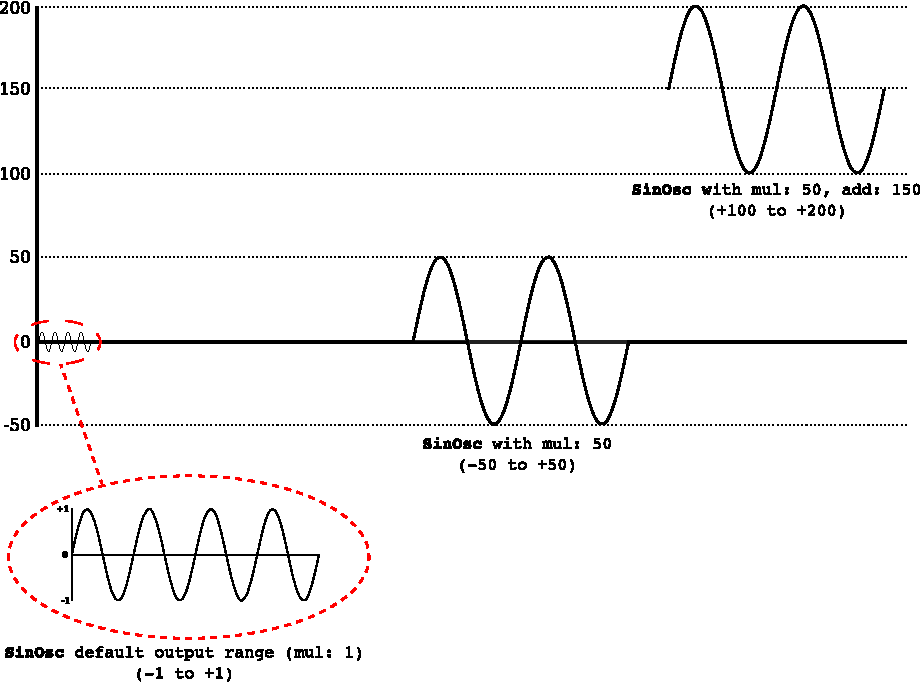
\includegraphics[scale=0.6]{fig-mul-add-scale.pdf}}}
\caption{Scaling UGen ranges with mul and add}
\label{fig:mul-add-scale}
\end{figure}

\subsection{\texttt{linlin} and friends}

For any other arbitrary scaling of ranges, you can use the handy methods \texttt{linlin}, \texttt{linexp}, \texttt{explin}, \texttt{expexp}. The method names hint at what they do: convert a linear range to another linear range (\texttt{linlin}), linear to exponential (\texttt{linexp}), etc.

\begin{lstlisting}[style=SuperCollider-IDE, basicstyle=\scttfamily\footnotesize]
// A bunch of numbers
a = [1, 2, 3, 4, 5, 6, 7];
// Rescale to 0-127, linear to linear
a.linlin(1, 7, 0, 127).round(1);
// Rescale to 0-127, linear to exponential
a.linexp(1, 7, 0.01, 127).round(1); // don't use zero for an exponential range
\end{lstlisting}

For a review of linear and exponential, look up online the difference between arithmetic and geometric sequences. Briefly, linear (arithmetic) sequences are like "1, 2, 3, 4, 5, 6" or "3, 6, 9, 12, 15", etc; and exponential (geometric) sequences are like "1, 2, 4, 8, 16, 32" or "3, 9, 27, 81, 243", etc.